\mysection{State-Space Analysis}
\label{sec:statespace}

  We analyze StreamIt programs at the filter level. We create a data
structure representation that fully describes a state space filter. We
parse the code of each StreamIt filter to determine whether or not it
is state space; if so we initialize a data structure, fill it with the
appropriate values through a process called \emph{extraction}, and
associate the structure with the filter. We provide a set of rules to
combine state space representations of filters in higher StreamIt
blocks---pipelines, splitjoins, and feedback loops. Such a process
results in a single 
\clearpage
\noindent state space representation for the entire block.  We also describe how
to \emph{expand} a representation so that it can be combined with
blocks of mis-matching dimensions.

\mysubsection{Representation}

    Our first task is to create a data structure that fully captures
the state space representation of a StreamIt filter.  We save a
filter's number of states, push rate, and pop rate in variables
which we term $s$, $u$, and $o$, respectively. Our data structure
also contains the matrices $\mathbf{A}$, $\mathbf{B}$,
$\mathbf{C}$, and $\mathbf{D}$ with dimensions $s \times s$, $s
\times o$, $u \times s$, and $u \times o$, respectively. The
inputs to a filter are denoted as $\vec{\mathbf{u}}$ (length $o$),
the outputs as $\vec{\mathbf{y}}$ (length $u$), and the states as
$\vec{\mathbf{x}}$ (length $s$). Upon every execution of the
filter, we can calculate the outputs by the formula
$\vec{\mathbf{y}} = \mathbf{C}\vec{\mathbf{x}} +
\mathbf{D}\vec{\mathbf{u}}$, and update the state matrix by the
formula $\vec{\dot{\mathbf{x}}} = \mathbf{A}\vec{\mathbf{x}} +
\mathbf{B}\vec{\mathbf{u}}$. For convenience, we will calculate
the filter outputs before updating the state matrix. Since the
states may have initial values other than zero, we store these
values as the vector $\overrightarrow{\mathbf{initVec}}$ (length
$s$).

    Since we have not included a constant term in our model, we
will set one of the state variables to be the constant $1$. This
variable will not be updated by any of the states or inputs, and
its initial value will be $1$, so it will always remain that
value. Any state or output that depends on a constant term can now
refer to a multiple of the constant state variable instead.

    As long as a filter's peek rate (which we term $e$) equals its pop
rate, the data structure as currently designed can fully represent
the filter. We must include additional modifications for a filter
with a peek rate greater than its pop rate. Note that such a
filter still removes $o$ items from its input tape upon every
execution, but it accesses $e-o$ additional items on its input
tape. Therefore, our current data structure would work as long as
there is some way to access these additional items.

    We solve the problem of having a peek rate greater than a pop
rate by storing $e-o$ items from the input tape in the state
vector $\vec{\mathbf{x}}$. Therefore, when a filter executes, it
can access all $e$ items it needs, $o$ items from its input vector
and $e-o$ items from its state vector. These $e-o$ states must be
updated by the inputs and themselves - the specifics are covered
in the next section. We store the number of states used for inputs
as the variable $stored$. This will be useful when combining
representations.

    When the filter is executed for the first time, it will have access
to the $o$ items in the input vector, but the $e-o$ states it
needs will be uninitialized from the input tape. Therefore, we
need to update the state vector before computing the output/state
update equation pair for every filter execution. We introduce two
new matrices, $\mathbf{A_{pre}}$ and $\mathbf{B_{pre}}$ to perform
this initialization. Before the filter runs it will perform the
state update $\vec{\dot{\mathbf{x}}} =
\mathbf{A_{pre}}\vec{\mathbf{x}} +
\mathbf{B_{pre}}\vec{\mathbf{u_{pre}}}$. The initialization input
vector, $\vec{\mathbf{u_{pre}}}$, has length $o_{pre} = e-o$. For
now, $o_{pre}$ and $stored$ have the same value, but combining
filters might result in $o_{pre}$ being greater than $stored$.
$\mathbf{A_{pre}}$ is $s \times s$ and $\mathbf{B_{pre}}$ is $s
\times o_{pre}$. Note that initial assignments of the state
variables by $\overrightarrow{\mathbf{initVec}}$ are done
immediately when a filter is created, while initialization by
$\mathbf{A_{pre}}$ and $\mathbf{B_{pre}}$ is afterwards, when
there are a sufficient number ($o_{pre}$) of items on the input
tape.

    Putting these pieces together, we find a full representation
consists of the push and pop rates, the number of state variables,
the number of stored inputs, the four state matrices, an initial
state vector, and possibly an initial pop rate and two
initialization state matrices. We define a state space
representation $\mathrm{R}$ as the tuple $\langle$$u$, $o$, $s$,
$stored$, $\mathbf{A}$, $\mathbf{B}$, $\mathbf{C}$, $\mathbf{D}$,
$\overrightarrow{\mathbf{initVec}}$, $\mathbf{A_{pre}}$,
$\mathbf{B_{pre}}$, $o_{pre}$$\rangle$. When we introduce a
representation $\mathrm{R_i}$, each of its values in the ordered
set will be denoted with the index $i$ (for example $u_i$,
$\mathbf{A_i}$). For representations of filters that do not need
the initialization matrices, we will write $\mathbf{A_{pre}} =
null$, $\mathbf{B_{pre}} = null$, $o_{pre} = 0$. In this case, the
filter will not have any stored inputs, so $stored = 0$ as well.

    Representations are initially created from StreamIt filters and
ultimately converted to StreamIt filters. Between these steps,
however, representations of the higher StreamIt block types can be
derived by combining the representations of their parts.  Therefore,
from now on we will say that a representation refers to a block rather
than a filter. The exception is in the following section, where we
discuss how to create a representation from a StreamIt filter.
% Hence we explicitly refer to a filter rather than block
%representation in that section.

\mysubsection{Extraction}

    We use a simple dataflow analysis to extract the state space representation of
a filter. We symbolically execute a single iteration of a filter's
work function, maintaining a vector pair representation for each
local variable and filter field variable that is encountered
(together, these are termed program variables). If the outputs and
field variables all have vector pair representations, then the
filter is state space linear, and the vectors are used as rows of
$\mathbf{A}$, $\mathbf{B}$, $\mathbf{C}$, and $\mathbf{D}$. 
%See \cite{Lamb}
%for a treatment of the linear case.

    We attempt to find a vector pair
($\vec{\mathbf{v}}$,$\vec{\mathbf{w}}$) for each program variable
$y$ where $y = \vec{\mathbf{v}} \cdot \vec{\mathbf{u}} +
\vec{\mathbf{w}} \cdot \vec{\mathbf{x}}$. $\vec{\mathbf{u}}$ is
the filter input vector and $\vec{\mathbf{x}}$ is the filter state
vector. When $y$ is on the left hand side of an assignment
statement, terms from the right hand side are compared with
entries from $\vec{\mathbf{u}}$ (inputs) and $\vec{\mathbf{x}}$
(states). The coefficients from terms that match are used for to
fill the corresponding entries in $\vec{\mathbf{v}}$ and
$\vec{\mathbf{w}}$, as long as they are constants. If any
coefficient is not a constant, then $y$ is non-linear.

    The input vector, $\vec{\mathbf{u}}$, is defined as $[peek(e-o)
~peek(e-o+1) ~... ~peek(o-1)]$. The state vector,
$\vec{\mathbf{x}}$, holds $e-o$ variables from the input tape
($peek(0) ~... ~peek(e-o-1)$), every field variable, and a
variable for the constant 1. We do not consider local variables
for the state vector, because their values are not saved across
filter executions. 
%Therefore, their values should be resolved to
%constants at compile time. 
A field variable has the initial vector
pair ($\vec{\mathbf{0}}$,$\left [
\begin{array} {ccccc} 0 & ... & 1 & ... & 0 \end{array} \right
]$), where the 1 corresponds to the field variable itself.

    If the vector pair can be found, then the program variable $y$ can
be written as a linear combination of the inputs and state
variables, with the vector pair entries representing the weights.
Then the final assignment to state variable $x_i$ by some program
variable $y_i$ indicates that the $i^{th}$ rows of $\mathbf{A}$
and $\mathbf{B}$ should be $\vec{\mathbf{w_i}}$ and
$\vec{\mathbf{v_i}}$, respectively. Similarly, the $j^{th}$ push
statement using program variable $y_j$ indicates that the $j^{th}$
rows of $\mathbf{C}$ and $\mathbf{D}$ should be
$\vec{\mathbf{w_j}}$ and $\vec{\mathbf{v_j}}$, respectively. For
the constant state variable $1$, the corresponding rows of
$\mathbf{A}$ and $\mathbf{B}$ are all zeros.

    We use the same procedure in the init function to find the initial
values for each field variable. However, we do not need a vector
$\vec{\mathbf{v}}$ for the inputs, since there are no inputs to
the init function. The initial value for each stored inputs is
zero, and the initial value for the variable $1$ is one.

    Finally, consider the stored input states (call them
$\vec{\mathbf{x_s}}$). They are updated by the inputs; however if
$stored > o$, then some of the input states must be updated by
other input states. In particular, the first $stored-o$ input
states are updated by the last $stored-o$ inputs, and the
remaining $o$ input states are updated by the $o$ inputs. The
update is described by the equation:
\starteqnstar
\vec{\dot{\mathbf{x_s}}} = \left [
\begin{array} {cc} \mathbf{0} & \mathbf{I} \\ \mathbf{0} &
\mathbf{0} \end{array} \right ] \vec{\mathbf{x_s}} + \left [
\begin{array} {c} \mathbf{0} \\ \mathbf{I} \end{array} \right ]
\vec{\mathbf{u}}
\doneeqnstar

    We also create initialization matrices to put values from the
input tape into the input states:
\starteqnstar
\vec{\dot{\mathbf{x_s}}} = \mathbf{0} \vec{\mathbf{x_s}} +
\mathbf{I} \vec{\mathbf{u_{pre}}}
\doneeqnstar

\vspace{-9pt} Stored inputs are always updated as shown in the same manner.
Therefore, we will use $\mathbf{A_s}$ and $\mathbf{B_s}$ to
describe this update, where the values of these two matrices are
shown in (3.1).

\mysubsubsection{Extraction Example}

Consider another IIR filter.  Unlike the example in
Section~\ref{sec:background}, this filter uses peeking to read
elements from the tape without consuming them.

\begin{singlespace}
\vspace{-12pt}
\small
\begin{verbatim}
float->float filter IIR() {
    float curr;  // example of a field variable
    work push 1 pop 1 peek 3 {
      float temp; // example of a local variable
      temp = (peek(0) + peek(1) + peek(2))/6;
      curr = temp + curr/2;
      push(curr);
      pop();
    }
}
\end{verbatim}
\vspace{-36pt}
\end{singlespace}
    The input vector is $\left [ \begin{array} {c} peek(2) \end{array}
\right ]$ and the state vector is $\left [ \begin{array} {c} \vspace{-36pt} \\ \vspace{-12pt} peek(0) \\ \vspace{-12pt}
peek(1) \\ \vspace{-12pt} curr \\ \vspace{-12pt} 1 \vspace{12pt} \end{array} \right ]$. The first program
variable encountered is $temp$. It is given the vector pair
($\left [ \begin{array} {c} 1/6 \end{array} \right ]$, $\left [
\begin{array} {cccc} 1/6 & 1/6 & 0 & 0 \end{array} \right ]$). The
variable $curr$, as a state variable, has an initial vector pair:
($\left [ \begin{array} {c} 0 \end{array} \right ]$, $\left
[\begin{array} {cccc} 0 & 0 & 1 & 0
\end{array} \right ]$). When $curr$ is found in an assignment
statement, it is given a new vector pair, constructed as $1$ times
the vector pair for $temp$ plus $1/2$ times the old vector pair
for $curr$: ($\left [ \begin{array} {c} 1/6 \end{array} \right ]$,
$\left [ \begin{array} {cccc} 1/6 & 1/6 & 1/2 & 0 \end{array}
\right ]$). The output is $curr$, so it is given the same vector
pair. The final pair for $curr$ represents its state update. The
stored inputs $peek(0)$, $peek(1)$ are updated as mentioned in
(3.1), and the constant $1$ is not updated. Therefore, we have:

\begin{minipage}{2.3in}
\starteqnstar
\mathbf{A} = \left [ \begin{array} {cccc} 0 & 1 & 0 & 0 \\ 0 &
0 & 0 & 0 \\ 1/6 & 1/6 & 1/2 & 0 \\ 0 & 0 & 0 & 0 \end{array}
\right ]
\doneeqnstar
\end{minipage}
\begin{minipage}{1.4in}
\starteqnstar
\mathbf{B} = \left [ \begin{array} {c} 0 \\ 1 \\ 1/6 \\ 0
\end{array} \right ]
\doneeqnstar
\end{minipage}
\begin{minipage}{2.3in}
\starteqnstar
\mathbf{C} = \left [ \begin{array} {cccc} 1/6 & 1/6 & 1/2 & 0
\end{array} \right ]
\doneeqnstar
\starteqnstar
\mathbf{D} = \left [ \begin{array} {c} 1/6 \end{array} \right ] \\
\doneeqnstar
\end{minipage}

\begin{minipage}{1.6in}
\starteqnstar
\overrightarrow{\mathbf{initVec}} = \left [ \begin{array} {c}
0 \\ 0 \\ 0 \\ 1 \end{array} \right ]
\doneeqnstar
\end{minipage}
\begin{minipage}{1.6in}
\starteqnstar
\mathbf{A_{pre}} = \left [ \begin{array} {cccc} 0 & 0 & 0 & 0 \\
0 & 0 & 0 & 0 \\ 0 & 0 & 1 & 0 \\ 0 & 0 & 0 & 1 \end{array}
\right ]
\doneeqnstar
\end{minipage}
\begin{minipage}{2.5in}
\starteqnstar
\mathbf{B_{pre}} = \left [ \begin{array} {cc} 1 & 0 \\ 0 & 1
\\ 0 & 0 \\ 0 & 0 \end{array} \right ] \\
\doneeqnstar
\end{minipage}

    The pop and push rates are both one, and we have four states so $o
= 1, u = 1, s = 4$. We have two stored input states, so $o_{pre} =
2, stored = 2$.

\mysubsection{Combination}

    If all blocks within a pipeline, splitjoin, or feedback loop have
state space representations, we can combine them into a single
representation using the rules developed in this section. We combine
blocks for two reasons.  First, combination can eliminate redundant
computations across blocks.  Second, combination exposes optimization
opportunities, as intra-block optimizations (described in
Section~\ref{sec:optimization}) can effectively be applied across
blocks by combining the blocks first.

\mysubsubsection{Pipeline}
\label{sec:pipeline}

    Consider two blocks connected in a pipeline with representations
$\mathrm{R_1}$ and $\mathrm{R_2}$. Let $\mathrm{R}$ denote the
combined representation of the two blocks, which we are trying to
derive. Suppose the output rate of $\mathrm{R_1}$ equals the input
rate of $\mathrm{R_2}$ ($u_1 = o_2$). If this is not the case, we must
expand one or both blocks to have their input/output rates match
($u_{1\_new} = o_{2\_new} = lcm(u_1,o_2)$). Block expansion is covered
in Section~\ref{sec:expansion}. Since the output of $\mathrm{R_1}$
($y_1$) is equivalent to the input of $\mathrm{R_2}$ ($u_2$), we can
write:

\begin{minipage}{3in}
\starteqnstar
\vec{\dot{\mathbf{x_1}}} & = & \mathbf{A_1}\vec{\mathbf{x_1}} + \mathbf{B_1}\vec{\mathbf{u_1}} \\
\vec{\dot{\mathbf{x_2}}} & = & \mathbf{A_2}\vec{\mathbf{x_2}} + \mathbf{B_2}\vec{\mathbf{y_1}}
\doneeqnstar
\end{minipage}
\begin{minipage}{3in}
\starteqnstar
\vec{\mathbf{y_1}} & = & \mathbf{C_1}\vec{\mathbf{x_1}} + \mathbf{D_1}\vec{\mathbf{u_1}} \\
\vec{\mathbf{y_2}} & = & \mathbf{C_2}\vec{\mathbf{x_2}} +
\mathbf{D_2}\vec{\mathbf{y_1}}
\doneeqnstar
\end{minipage}

Substituting for $\vec{\mathbf{y_1}}$ we get:
\starteqnstar
\vec{\dot{\mathbf{x_2}}} & = & \mathbf{A_2}\vec{\mathbf{x_2}} + \mathbf{B_2}(\mathbf{C_1}\vec{\mathbf{x_1}} + \mathbf{D_1}\vec{\mathbf{u_1}}) \\
\vec{\mathbf{y_2}} & = & \mathbf{C_2}\vec{\mathbf{x_2}} +
\mathbf{D_2}(\mathbf{C_1}\vec{\mathbf{x_1}} +
\mathbf{D_1}\vec{\mathbf{u_1}})
\doneeqnstar

Which simplifies to:
\starteqnstar
\vec{\dot{\mathbf{x_2}}} & = & \mathbf{A_2}\vec{\mathbf{x_2}} + \mathbf{B_2}\mathbf{C_1}\vec{\mathbf{x_1}} + \mathbf{B_2}\mathbf{D_1}\vec{\mathbf{u_1}} \\
\vec{\mathbf{y_2}} & = & \mathbf{C_2}\vec{\mathbf{x_2}} +
\mathbf{D_2}\mathbf{C_1}\vec{\mathbf{x_1}} +
\mathbf{D_2}\mathbf{D_1}\vec{\mathbf{u_1}}
\doneeqnstar

Let $\vec{\mathbf{x}} = \left [ \begin{array} {c} \vec{\mathbf{x_1}} \\
\vec{\mathbf{x_2}} \end{array} \right ]$, $\vec{\mathbf{u}} =
\vec{\mathbf{u_1}}$ (the input to the entire pipeline), and
$\vec{\mathbf{y}} = \vec{\mathbf{y_2}}$ (the output of the entire
pipeline). The equations relating $\vec{\mathbf{x}}$,
$\vec{\mathbf{u}}$, and $\vec{\mathbf{y}}$ are:
\starteqnstar
\vec{\dot{\mathbf{x}}} & = & \mathbf{A}\vec{\mathbf{x}} + \mathbf{B}\vec{\mathbf{u}} \\
\vec{\mathbf{y}} & = & \mathbf{C}\vec{\mathbf{x}} + \mathbf{D}\vec{\mathbf{u}}
\doneeqnstar
\starteqnstar 
\mathbf{A} = \left [ \begin{array} {cc} \mathbf{A_1} &
\mathbf{0} \\ \mathbf{B_2}\mathbf{C_1} & \mathbf{A_2} \end{array} \right ] ~~~~~
\mathbf{B} = \left [ \begin{array} {c} \mathbf{B_1} \\ \mathbf{B_2}\mathbf{D_1} \end{array} \right ] ~~~~~
\mathbf{C} = \left [ \begin{array} {cc} \mathbf{D_2}\mathbf{C_1} & \mathbf{C_2} \end{array} \right ] ~~~~~
\mathbf{D} = \mathbf{D_2}\mathbf{D_1}
\doneeqnstar

    The input to the pipeline is identical to the input to $\mathrm{R_1}$,
and the output of the pipeline is identical to the output of
$\mathrm{R_2}$. Furthermore, the states of the pipeline are the
states of the first block appended to the states of the second
block. Therefore, $u = u_2$, $o = o_1$, $s = s_1 + s_2$,
$\overrightarrow{\mathbf{initVec}} = \left [ \begin{array} {c}
\overrightarrow{initVec_1} \\ \overrightarrow{initVec_2}
\end{array} \right ]$.

    If both blocks do not have initialization matrices, then the entire
pipeline does not need initialization matrices, so
$\mathbf{A_{pre}} = null$, $\mathbf{B_{pre}} = null$, $o_{pre} =
0$, $stored = 0$. If only the first block has initialization
matrices, then we want to initialize the states in the pipeline
corresponding to the first block while keeping the states
corresponding to the second block unchanged. Therefore:
\starteqnstar
\mathbf{A_{pre}} = \left [ \begin{array} {cc}
\mathbf{A_{pre1}} & \mathbf{0} \\ \mathbf{0} & \mathbf{I} \end{array} \right ] ~~~~~
\mathbf{B_{pre}} = \left [ \begin{array} {c} \mathbf{B_{pre1}} \\ \mathbf{0} \end{array} \right ] ~~~~~
o_{pre} = o_{pre1} ~~~~~
stored = stored_1
\doneeqnstar

    If the second block has initialization matrices, we must run the
first block enough times to provide the necessary inputs to initialize
the second block. However, this might result in the first block
providing extra initial inputs to the second block. In that case, we
must change the representation of the second block to increase its
number of stored inputs.  A full description of this case appears
in~\cite{Agrawal04}.

%%  (the way to do this is
%% covered in Section 3.4.2). Suppose this is done and the first
%% block must run $n$ times (along with its initialization matrices,
%% if it has them) to initialize the second block. Denote
%% $\mathbf{{A_1}^e}$, $\mathbf{{B_1}^e}$, $\mathbf{{C_1}^e}$, and
%% $\mathbf{{D_1}^e}$ as the matrices that describe running the first
%% block $n$ times (see Equations (3.6)-(3.9)). Then the
%% initialization of the entire pipeline is derived by combining
%% these matrices with $\mathbf{A_{pre2}}$, $\mathbf{B_{pre2}}$ just
%% as the $\mathbf{A}$, $\mathbf{B}$, $\mathbf{C}$, and $\mathbf{D}$
%% matrices are combined for the two blocks:
%% \starteqnstar
%% \mathbf{A_{pre}} & = & \left [ \begin{array} {cc}
%% \mathbf{{A_1}^e} & \mathbf{0} \\
%% \mathbf{B_{pre2}} \mathbf{{C_1}^e} & \mathbf{A_{pre2}} \end{array} \right ] \\
%% \mathbf{B_{pre}} & = & \left [ \begin{array} {c}
%% \mathbf{{B_1}^e} \\ \mathbf{B_{pre2}} \mathbf{{D_1}^e} \\ \end{array} \right ] \\
%% o_{pre} & = & o_{pre1} + n*o_1 \\
%% stored & = & stored_1
%% \doneeqnstar

    If there are more than two blocks in a pipeline, we collapse
the pipeline in the following manner: combine the first two blocks
to get one block representation, combine this with the third
block, etc.

\mysubsubsection{Splitjoin and Feedback Loop}

The combination rules for splitjoins and feedback loops are somewhat
involved, and we omit them due to space considerations.  An important
benefit of a linear state space representation over a linear
representation is that feedback loops can be collapsed; the items on
the feedback path become states in the combined block.  A thorough
treatment of these cases appears in~\cite{Agrawal04}.

%%     There are two types of splitjoins - those with roundrobin and
%% duplicate splitters. In order to collapse the branches of a
%% splitjoin to a single representation, we need the splitjoin to
%% have a duplicate splitter, because then the representation in each
%% branch accesses the same inputs. Therefore, for roundrobin
%% splitjoins we first detail a procedure to convert to a duplicate
%% splitjoin. Then we describe how to create a representation of a
%% duplicate splitjoin.

%% \subsubsubsection{Conversion from roundrobin to duplicate splitjoin}

%%     Suppose the roundrobin splitjoin has $k$ branches and let $w_i$ and
%% $\mathrm{M_i}$ denote the splitter weight and state space
%% representation, respectively, on the $i^{th}$ branch. In each
%% branch $i$ we add a filter with representation $\mathrm{L_i}$ that
%% outputs to $\mathrm{M_i}$ in a pipeline format. Since the
%% splitjoin now has a duplicate splitter, $\mathrm{M_i}$ receives
%% every input element to the entire splitjoin. In order to exactly
%% simulate the original roundrobin splitter, $\mathrm{M_i}$ should
%% only see $w_i$ elements for every $\sum_{j=1}^{k} w_j$ input
%% elements to the splitjoin. Therefore, we make $\mathrm{L_i}$ input
%% $\sum_{j=1}^{k} w_j$ elements and output $w_i$ elements. In
%% particular, $\mathrm{L_i}$ ignores the first $\sum_{j=1}^{i-1}
%% w_j$ inputs (which correspond to inputs to the previous branches),
%% outputs the next $w_i$ inputs (which correspond to inputs to the
%% $i^{th}$ branch), and ignores the remaining $\sum_{j=i+1}^{k} w_j$
%% inputs\footnote{In DSP terminology, $\mathrm{L_i}$ is called a
%% downsampler.} (which correspond to inputs to the later branches).

%%     The values for $\mathrm{L_i}$ are $o = \sum_{j=1}^{k} w_j$, $u = w_i$,
%% $s = 1$, $\mathbf{A} = \mathbf{0}$, $\mathbf{B} = \mathbf{0}$,
%% $\mathbf{C} = \mathbf{0}$, $\mathbf{D} = \left [ \begin{array}
%% {ccc} \mathbf{0} & \mathbf{I} & \mathbf{0} \end{array} \right ]$,
%% $\overrightarrow{\mathbf{initVec}} = \vec{\mathbf{0}}$,
%% $\mathbf{A_{pre}}, \mathbf{B_{pre}} = null$, $o_{pre} = 0$,
%% $stored = 0$. We use one state in the representation, even though
%% none are needed, to make combinations of representations simpler.
%% Once $\mathrm{L_i}$ is created, it can be combined with
%% $\mathrm{M_i}$ to form a single representation (call it
%% $\mathrm{R_i}$).

%% \subsubsubsection{Collapsing duplicate splitjoins}

%%     Let $\mathrm{R}$ be the representation for the entire
%% splitjoin, $\mathrm{R_i}$ be the representation on the $i^{th}$
%% branch, $k$ be the number of branches. In order to combine the
%% branch representations, we must derive a steady-state execution of
%% the entire splitjoin. Denote the joiner weight of each branch $i$
%% as $w_i$ (note that we used $w_i$ earlier to denote a splitter
%% weight). Each branch outputs $u_i$ items but $w_i$ items from that
%% branch are needed to execute the splitjoin once. $\mathrm{R_i}$
%% can be expanded to output $lcm(u_i,w_i)$ items, which would result
%% in $\frac{lcm(u_i,w_i)}{w_i}$ splitjoin executions. This means we
%% must execute the splitjoin a multiple of
%% $\frac{lcm(u_1,w_1)}{w_1}$ times to satisfy the constraints of the
%% first branch, a multiple of $\frac{lcm(u_2,w_2)}{w_2}$ times to
%% satisfy the constraints of the second branch, etc. Therefore, we
%% shall construct $\mathrm{R}$ to execute the splitjoin
%% $lcm(\frac{lcm(u_1,w_1)}{w_1},\frac{lcm(u_2,w_2)}{w_2},...,\frac{lcm(u_k,w_k)}{w_k})$
%% times. Call this value $E$. Each representation $\mathrm{R_i}$
%% must output $w_i * E$ elements, so $\mathrm{R_i}$ must be expanded
%% $\frac{w_i * E}{u_i}$ times.

%%     After these expansions, each branch representation  should now
%% have the same input rate $o_i$. If not, the splitjoin is
%% ill-formed and cannot be compiled by StreamIt. Since these
%% representations will be combined, we need each to have the same
%% number of stored inputs and the same initial pop rate. To satisfy
%% both constraints, we increase the number of stored inputs in each
%% representation to the value $max(stored_i,o_{prei})$ over all $i$.

%%     Now that the branch representations have been standardized,
%% they can be combined to a single representation. The stored input
%% states in each representation evolve in the same manner, so only
%% one set of them is needed for the entire splitjoin representation.
%% Let $\vec{\mathbf{x_i}} = \left [ \begin{array} {c}
%% \vec{\mathbf{x_{is}}} \\ \vec{\mathbf{x_{ir}}} \end{array} \right
%% ]$, where $\vec{\mathbf{x_{is}}}$ and $\vec{\mathbf{x_{ir}}}$ are
%% the stored input states and remaining states of $\mathrm{R_i}$,
%% respectively. For each representation $i$ denote the state space
%% equation pair as:
%% \starteqnstar
%% \left [ \begin{array} {c} \vec{\dot{\mathbf{x_{is}}}} \\
%% \vec{\dot{\mathbf{x_{ir}}}} \end{array} \right ] & = & \left [
%% \begin{array} {cc} \mathbf{A_{is}} & \mathbf{0} \\
%% \mathbf{A_{irs}} & \mathbf{A_{irr}} \end{array} \right ] \left [
%% \begin{array} {c} \vec{\mathbf{x_{is}}} \\ \vec{\mathbf{x_{ir}}}
%% \end{array} \right ] +  \left [ \begin{array} {c} \mathbf{B_{is}}
%% \\ \mathbf{B_{ir}} \end{array} \right ] \vec{\mathbf{u}} \\
%% \vec{\mathbf{y}} & = & \left [ \begin{array} {cc} \mathbf{C_{is}}
%% & \mathbf{C_{ir}} \end{array} \right ] \left [ \begin{array} {c}
%% \vec{\mathbf{x_{is}}} \\ \vec{\mathbf{x_{ir}}} \end{array} \right
%% ] + \mathbf{D} \vec{\mathbf{u}}
%% \doneeqnstar

%%     Since the stored input states in each representation are
%% equivalent, we set them to be $\vec{\mathbf{x_s}}$, and set their
%% corresponding matrix blocks to be $\mathbf{A_s}$ and
%% $\mathbf{B_s}$. Let $\vec{\mathbf{x}} = \left [ \begin{array} {c}
%% \vec{\mathbf{x_{s}}} \\ \vec{\mathbf{x_{1r}}} \\
%% \vec{\mathbf{x_{2r}}} \\ ... \\ \vec{\mathbf{x_{kr}}} \end{array}
%% \right ]$. The states $\vec{\mathbf{x_{ir}}}$ evolve separately,
%% so:
%% \starteqnstar
%% \mathbf{A} & = & \left [ \begin{array} {ccccc} \mathbf{A_s} &
%% \mathbf{0} & \mathbf{0} & ... & \mathbf{0} \\ \mathbf{A_{1rs}} &
%% \mathbf{A_{1rr}} & \mathbf{0} & ... & \mathbf{0} \\
%% \mathbf{A_{2rs}} & \mathbf{0} & \mathbf{A_{2rr}} & ... & \mathbf{0}
%% \\ ... & ... & ... & ... \\ \mathbf{A_{krr}} & \mathbf{0} &
%% \mathbf{0} & ... & \mathbf{A_{krs}} \end{array} \right ] \\
%% \mathbf{B} & = & \left [ \begin{array} {c} \mathbf{B_s} \\ \mathbf{B_{1r}} \\
%% \mathbf{B_{2r}} \\ ... \\ \mathbf{B_{kr}} \end{array} \right ]
%% \doneeqnstar

%%     Similarly for the initialization matrices we have:
%% \starteqnstar
%% \mathbf{A_{pre}} & = & \left [ \begin{array} {ccccc} \mathbf{0} &
%% \mathbf{0} & \mathbf{0} & ... & \mathbf{0} \\
%% \mathbf{0} & \mathbf{A_{pre1rr}} & \mathbf{0} & ... & \mathbf{0} \\
%% \mathbf{0} & \mathbf{0} & \mathbf{A_{pre2rr}} & ... & \mathbf{0} \\
%% ... & ... & ... & ... & ... \\ \mathbf{0} & \mathbf{0} &
%% \mathbf{0} & ... & \mathbf{A_{prekrr}} \end{array} \right ] \\
%% \mathbf{B_{pre}} & = & \left [ \begin{array} {c} \mathbf{B_{pres}} \\
%% \mathbf{B_{pre1r}} \\ \mathbf{B_{pre2r}} \\ ... \\
%% \mathbf{B_{prekr}} \end{array} \right ]
%% \doneeqnstar

%%     These equations are simpler because $\mathbf{A_{pres}} =
%% \mathbf{0}$ and $\mathbf{A_{preirs}} = \mathbf{0}$.

%%     In order to simulate the roundrobin nature of the joiner,
%% we must output $w_1$ items from $\mathrm{R_1}$, then $w_2$ items
%% from $\mathrm{R_2}$, up to $w_k$ items from $\mathrm{R_k}$, and
%% repeat this process $E$ times (because we are running the
%% splitjoin $E$ times). Let $\mathbf{C_i} = \left [
%% \begin{array} {cc} \mathbf{C_{is1}} & \mathbf{C_{ir1}} \\
%% \mathbf{C_{is2}} & \mathbf{C_{ir2}} \\ ... & ... \\
%% \mathbf{C_{isexecutions}} & \mathbf{C_{irexecutions}} \end{array}
%% \right ]$, where $\left [ \begin{array} {cc} \mathbf{C_{isj}} &
%% \mathbf{C_{irj}} \end{array} \right ]$ is $w_i \times s_i$. Let
%% $\mathbf{D_i} = \left [
%% \begin{array} {c} \mathbf{D_{i1}} \\ \mathbf{D_{i2}} \\ ... \\
%% \mathbf{D_{iexecutions}} \end{array} \right ]$, where
%% $\mathbf{D_{ij}}$ is $w_i \times o$. Then we have:
%% \starteqnstar
%% \mathbf{C} & = & \left [ \begin{array} {ccccc} \mathbf{C_{1s1}} &
%% \mathbf{C_{1r1}} & \mathbf{0} & ... & \mathbf{0} \\
%% \mathbf{C_{2s1}} & \mathbf{C_{2r1}} & \mathbf{0} & ... &
%% \mathbf{0} \\ ... & ... & ... & ... & ... \\ \mathbf{C_{ks1}} &
%% \mathbf{0} & \mathbf{0} & ... & \mathbf{C_{kr1}} \\ ... & ... & ... & ... & ... \\
%% \mathbf{C_{1sk}} & \mathbf{C_{1rk}} & \mathbf{0} & ... & \mathbf{0} \\
%% \mathbf{C_{2sk}} & \mathbf{C_{2rk}} & \mathbf{0} & ... & \mathbf{0} \\
%% ... & ... & ... & ... \\ \mathbf{C_{ksk}} & \mathbf{0} & \mathbf{0} & ... & \mathbf{C_{krk}}
%% \end{array} \right ] \\
%% \mathbf{D} & = & \left [ \begin{array} {c} \mathbf{D_{11}} \\
%% \mathbf{D_{21}} \\ ... \\ \mathbf{D_{k1}} \\ ... \\ \mathbf{D_{1k}} \\
%% \mathbf{D_{2k}} \\ ... \\ \mathbf{D_{kk}} \end{array} \right ]
%% \doneeqnstar

%%     We have derived $\mathbf{A}$, $\mathbf{B}$, $\mathbf{C}$,
%% $\mathbf{D}$, $\mathbf{A_{pre}}$, and $\mathbf{B_{pre}}$. As
%% mentioned previously, all the pop rates are equal so $o = o_1$.
%% Additionally, all the initial pop rates and stored inputs are
%% equal, so $o_{pre} = o_{pre1}$ and $stored = o_{pre1}$. The
%% splitjoin runs $E$ times, hence $u = E * \sum_{j=1}^{k} w_j$. The
%% states of the entire representation are the non-stored input
%% states of each branch representation concatenated along with one
%% set of the stored input states. Let $s_{ir}$ be the number of
%% non-stored input states in representation $i$ and let
%% $\overrightarrow{\mathbf{initVec_{ir}}}$ be the initial values of
%% these states. Then $s = stored + \sum_{j=1}^{k} s_{jr}$ and
%% $\overrightarrow{\mathbf{initVec}} =
%% \left [ \begin{array} {c} \vec{\mathbf{0}} \\ \overrightarrow{\mathbf{initVec_{1r}}} \\
%% \overrightarrow{\mathbf{initVec_{2r}}} \\ ... \\
%% \overrightarrow{\mathbf{initVec_{kr}}} \end{array} \right ]$.

%% \mysubsubsection{Feedback Loop}

%%     Recall that a feedback loop has a loop block and a body block.
%% Outputs from the body block and inputs to the entire feedback loop
%% are combined via a joiner to form the inputs to the loop block.
%% Outputs from the loop block are used as outputs of the entire
%% feedback loop and inputs of the loop block via a splitter.

%%     Let the loop block have representation $\mathrm{R_1}$, the body
%% block have representation $\mathrm{R_2}$, and the entire feedback
%% loop have representation $\mathrm{R}$. If the splitter is a
%% roundrobin one, we convert it to a duplicate one by adding the
%% appropriate downsamplers to the output branches, as described in
%% Section 3.3.2. The output branches of a feedback loop splitter
%% lead to the loop block and the output of the entire feedback loop.
%% Therefore, one downsampler must be placed before the loop block in
%% a pipeline format, and one downsampler must be placed after the
%% feedback loop in a pipeline format. The first downsampler and loop
%% block is combined to form a new loop block. The second downsampler
%% can be combined with the feedback loop after the feedback loop's
%% representation is computed.

%%     As in the case of a splitjoin, we must derive a steady-state
%% execution of the entire feedback loop in order to combine the loop
%% and body blocks. First we match the output rate of the body block
%% ($o_2$) with the input rate of the loop block ($u_1$) by expanding
%% the two representations appropriately. Now consider the roundrobin
%% joiner, and let $w_1$, $w_2$ be the weights on the branches from
%% the loop block and input to the body block, respectively. The loop
%% block outputs $u_1$ items, but $w_1$ items are needed to run the
%% feedback loop once. Therefore, the loop block can be expanded to
%% output $lcm(u_1,w_1)$ items, which would result in
%% $\frac{lcm(u_1,w_1)}{w_1}$ feedback loop executions. Call this
%% value $E$. The loop block is expanded to run
%% $\frac{lcm(u_1,w_1)}{u_1}$ times, and the body block is expanded
%% by this amount as well, since we still want the output rate of the
%% body block to equal the input rate of the loop block. Since the
%% feedback loop runs $E$ times, the body block receives $E*(w_1 +
%% w_2)$ inputs, which should equal the input rate of the expanded
%% body block. If not, the feedback loop is ill-formed.

%%     Once the above expansions are implemented, the feedback loop
%% is run by executing the loop and body blocks alternately. However,
%% the loop block depends on outputs from the body block, and the
%% body block depends on outputs from the loop block. In order to
%% begin execution of the entire feedback loop, there must be items
%% enqueued on the output tape of the loop block. The minimal number
%% of enqueued items is $u_1$, the output rate of the loop block.
%% However, there can be more enqueued items. We create a new
%% representation $\mathrm{R_3}$ that stores the enqueued values.
%% Upon each execution $\mathrm{R_3}$ inputs $u_1$ items from the
%% loop block and outputs $u_1$ items to the body block. It has one
%% state for each enqueued item. The equations for $\mathrm{R_3}$
%% are:
%% \starteqnstar
%% \vec{\dot{\mathbf{x_3}}} & = & \left [ \begin{array} {cc}
%% \mathbf{0} & \mathbf{I} \\ \mathbf{0} & \mathbf{0} \end{array} \right ]
%% \vec{\mathbf{x_3}} + \left [ \begin{array} {c} \mathbf{0} \\ \mathbf{I}
%% \end{array} \right ] \vec{\mathbf{u_3}} \\
%% \vec{\mathbf{y_3}} & = & \left [ \begin{array} {c} \mathbf{I} \\
%% \mathbf{0} \end{array} \right ] \vec{\mathbf{x_1}}
%% \doneeqnstar

%%     $\mathrm{R_3}$ does not have initialization matrices, and
%% $\overrightarrow{\mathbf{initVec_3}}$ is assigned the enqueued
%% values.

%%     Note that the output $\vec{\mathbf{y_3}}$ does not depend on
%% the input $\vec{\mathbf{u_3}}$. This is the key to starting the
%% feedback loop: $\mathrm{R_3}$ outputs first, the body block uses
%% these outputs along with inputs to the entire feedback loop to
%% execute and produce outputs, the loop body uses these outputs to
%% execute and produce outputs, $\mathrm{R_3}$ uses these outputs to
%% execute and produce outputs, etc.

%% \begin{figure}[bthp]
%%   \centering
%%   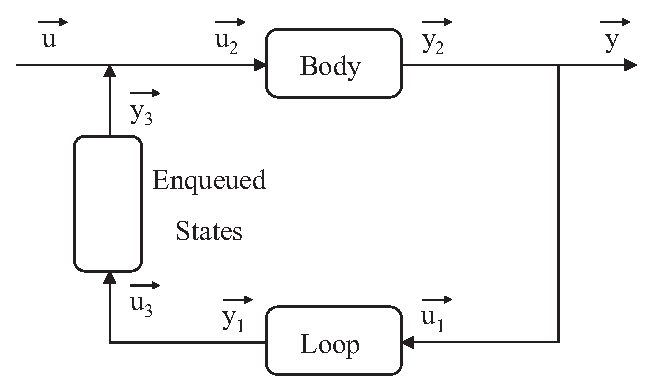
\includegraphics[width=3.0in]{figures/feedback2.eps}
%%   \caption{Labelled feedback loop}
%%   \label{fig:feedback2}
%% \end{figure}

%%     From figure \ref{fig:feedback2} it is apparent that $\vec{\mathbf{u_3}} =
%% \vec{\mathbf{y_1}}$, $\vec{\mathbf{y}} = \vec{\mathbf{y_2}} =
%% \vec{\mathbf{u_1}}$, and $\vec{\mathbf{u_2}}$ is composed of
%% $\vec{\mathbf{u}}$ and $\vec{\mathbf{u_3}}$. We can write the
%% equations for the body block as:
%% \starteqnstar
%% \vec{\dot{\mathbf{x_2}}} & = & \mathbf{A_2} \vec{\mathbf{x_2}} +
%% \mathbf{B_2} \vec{\mathbf{u_2}} = \mathbf{A_2}\vec{\mathbf{x_2}} +
%% \mathbf{B_{2\_1}} \vec{\mathbf{u}} + \mathbf{B_{2\_2}}
%% \vec{\mathbf{y_3}} = \mathbf{A_2}\vec{\mathbf{x_2}} +
%% \mathbf{B_{2\_1}} \vec{\mathbf{u}} + \mathbf{B_{2\_2}}
%% \mathbf{C_3} \vec{\mathbf{x_3}} \\
%% \vec{\mathbf{y_2}} & = & \mathbf{C_2} \vec{\mathbf{x_2}} +
%% \mathbf{D_2} \vec{\mathbf{u_2}} = \mathbf{C_2}\vec{\mathbf{x_2}} +
%% \mathbf{D_{2\_1}} \vec{\mathbf{u}} + \mathbf{D_{2\_2}}
%% \vec{\mathbf{y_3}} = \mathbf{C_2}\vec{\mathbf{x_2}} +
%% \mathbf{D_{2\_1}} \vec{\mathbf{u}} + \mathbf{D_{2\_2}}
%% \mathbf{C_3} \vec{\mathbf{x_3}}
%% \doneeqnstar

%%     Since $\vec{\mathbf{y}} = \vec{\mathbf{y_2}}$, we have written
%% the output of the feedback loop and the update for
%% $\vec{\mathbf{x_2}}$ in terms of the input to the feedback loop
%% and the state vectors. For the updates to $\vec{\mathbf{x_1}}$ and
%% $\vec{\mathbf{x_3}}$ we can write:
%% \starteqnstar
%% \vec{\dot{\mathbf{x_1}}} & = & \mathbf{A_1} \vec{\mathbf{x_1}} +
%% \mathbf{B_1} \vec{\mathbf{u_1}} = \mathbf{A_1}\vec{\mathbf{x_1}} +
%% \mathbf{B_1} \vec{\mathbf{y}} =  \mathbf{A_1}\vec{\mathbf{x_1}} +
%% \mathbf{B_1}(\mathbf{C_2}\vec{\mathbf{x_2}} + \mathbf{D_{2\_1}}
%% \vec{\mathbf{u}} + \mathbf{D_{2\_2}} \mathbf{C_3}
%% \vec{\mathbf{x_3}}) \\
%% & = & \mathbf{A_1}\vec{\mathbf{x_1}} +
%% \mathbf{B_1}\mathbf{C_2}\vec{\mathbf{x_2}} + \mathbf{B_1}
%% \mathbf{D_{2\_1}} \vec{\mathbf{u}} + \mathbf{B_1}
%% \mathbf{D_{2\_2}} \mathbf{C_3} \vec{\mathbf{x_3}} \\ \\
%% \vec{\dot{\mathbf{x_3}}} & = & \mathbf{A_3} \vec{\mathbf{x_3}} +
%% \mathbf{B_3} \vec{\mathbf{u_3}} = \mathbf{A_3}\vec{\mathbf{x_3}} +
%% \mathbf{B_3} \vec{\mathbf{y_1}} =  \mathbf{A_3}\vec{\mathbf{x_3}}
%% + \mathbf{B_3}(\mathbf{C_1}\vec{\mathbf{x_1}} + \mathbf{D_1}
%% \vec{\mathbf{u_1}}) \\
%% & = & \mathbf{A_3}\vec{\mathbf{x_3}} +
%% \mathbf{B_3}(\mathbf{C_1}\vec{\mathbf{x_1}} +
%% \mathbf{D_1}\vec{\mathbf{y}}) = \mathbf{A_3}\vec{\mathbf{x_3}} +
%% \mathbf{B_3}(\mathbf{C_1}\vec{\mathbf{x_1}} +
%% \mathbf{D_1}(\mathbf{C_2}\vec{\mathbf{x_2}} + \mathbf{D_{2\_1}}
%% \vec{\mathbf{u}} + \mathbf{D_{2\_2}} \mathbf{C_3}
%% \vec{\mathbf{x_3}})) \\
%% & = & \mathbf{A_3}\vec{\mathbf{x_3}} +
%% \mathbf{B_3}\mathbf{C_1}\vec{\mathbf{x_1}} +
%% \mathbf{B_3}\mathbf{D_1}\mathbf{C_2}\vec{\mathbf{x_2}} +
%% \mathbf{B_3}\mathbf{D_1}\mathbf{D_{2\_1}} \vec{\mathbf{u}} +
%% \mathbf{B_3}\mathbf{D_1}\mathbf{D_{2\_2}} \mathbf{C_3}
%% \vec{\mathbf{x_3}}
%% \doneeqnstar

%%     For the input and output rates we have $o = E * w_2$
%% and $u = u_2$. We use the states of all three representations, so
%% $s = s_1 + s_2 + s_3$ and $\overrightarrow{\mathbf{initVec}} =
%% \left [ \begin{array} {c} \overrightarrow{\mathbf{initVec_1}} \\
%% \overrightarrow{\mathbf{initVec_2}} \\
%% \overrightarrow{\mathbf{initVec_3}} \end{array} \right ]$. For
%% simplicity, we do not consider a loop or body block with
%% initialization matrices.

\mysubsection{Expanding a Representation}
\label{sec:expansion}

    We may want to run a block multiple times in order to
properly combine it with other blocks. For example, suppose block
$B_1$ inputs three items and outputs two items, and block $B_2$
inputs five items and outputs seven items. In order to combine
these blocks in a pipeline, $B_1$ must run five times (in order to
output ten items) and $B_2$ must run two times (in order to input
ten items). Therefore, we need to have a method to expand a
representation so that it models a block running multiple times,
rather than once.

    Consider the state space equation pair, where $\vec{\mathbf{u_1}}$ and
$\vec{\mathbf{y_1}}$ are the first set of inputs and outputs, and
$\vec{\mathbf{x}}$ is the original state vector: \vspace{-28pt}
\starteqnstar
\vec{\dot{\mathbf{x}}} & = & \mathbf{A}\vec{\mathbf{x}} + \mathbf{B}\vec{\mathbf{u_1}} \\
\vec{\mathbf{y_1}} & = & \mathbf{C}\vec{\mathbf{x}} +
\mathbf{D}\vec{\mathbf{u_1}}
\doneeqnstar

\vspace{-6pt} If we run the block again, the equation pair in terms of the
original state vector $\vec{\mathbf{x}}$ and the next set of
inputs and outputs ($\vec{\mathbf{u_2}}$ and $\vec{\mathbf{y_2}}$)
is:
\starteqnstar
\vec{\dot{\mathbf{x}}} & = & \mathbf{A}(\mathbf{A}\vec{\mathbf{x}}
+
\mathbf{B}\vec{\mathbf{u_1}}) + \mathbf{B}\vec{\mathbf{u_2}} \\
\vec{\mathbf{y_2}} & = & \mathbf{C}(\mathbf{A}\vec{\mathbf{x}} +
\mathbf{B}\vec{\mathbf{u_1}}) + \mathbf{D}\vec{\mathbf{u_2}}
\doneeqnstar

~ \vspace{-36pt} \\ \noindent Simplifying yields: \vspace{-12pt} 

\starteqnstar
\vec{\dot{\mathbf{x}}} & = & \mathbf{A}^2\vec{\mathbf{x}} +
\mathbf{AB}\vec{\mathbf{u_1}} + \mathbf{B}\vec{\mathbf{u_2}} \\
\vec{\mathbf{y_2}} & = & \mathbf{CA}\vec{\mathbf{x}} +
\mathbf{CB}\vec{\mathbf{u_1}} + \mathbf{D}\vec{\mathbf{u_2}}
\doneeqnstar

    Let $\vec{\mathbf{u}}$ be the combined input vector
($\vec{\mathbf{u}} = \left [ \begin{array} {c} \vec{\mathbf{u_1}}
\\ \vec{\mathbf{u_2}} \end{array} \right ]$) and $\vec{\mathbf{y}}$ be the combined output vector
($\vec{\mathbf{y}} = \left [ \begin{array} {c} \vec{\mathbf{y_1}}
\\ \vec{\mathbf{y_2}} \end{array} \right ]$). The representation in terms of these two
vectors is:
\starteqnstar
\vec{\dot{\mathbf{x}}} & = & \mathbf{A_2}\vec{\mathbf{x}} + \mathbf{B_2}\vec{\mathbf{u}} \\
\vec{\mathbf{y}} & = & \mathbf{C_2}\vec{\mathbf{x}} + \mathbf{D_2}\vec{\mathbf{u}}
\doneeqnstar
\starteqnstar
\mathbf{A_2} = \mathbf{A}^2 ~~~~~
\mathbf{B_2} = \left [ \begin{array} {cc} \mathbf{AB} & \mathbf{B} \end{array} \right ]  ~~~~~
\mathbf{C_2} = \left [ \begin{array} {c} \mathbf{C} \\
\mathbf{CA} \end{array} \right ] ~~~~~
\mathbf{D_2} = \left [ \begin{array} {cc} \mathbf{D} & \mathbf{0} \\
\mathbf{CB} & \mathbf{D} \end{array} \right ]
\doneeqnstar

    This new representation corresponds to a block that upon
every execution runs the old block twice. By induction, a general
formula for running a block n times is:
\starteqnstar
\mathbf{A_n} = \mathbf{A}^n ~~~~~
\mathbf{B_n} = \left [ \begin{array} {ccccc} \mathbf{A}^{n-1}
\mathbf{B} & \mathbf{A}^{n-2} \mathbf{B} & ...  & \mathbf{AB} &
\mathbf{B} \end{array} \right ]
\doneeqnstar
\starteqnstar
\mathbf{C_n} = \left [ \begin{array} {c} \mathbf{C} \\
\mathbf{CA} \\
... \\
\mathbf{CA^{n-2}} \\
\mathbf{CA^{n-1}} \end{array} \right ] ~~~~~
\mathbf{D_n} = \left [ \begin{array} {ccccccc}
\mathbf{D} & \mathbf{0} & \mathbf{0} & ... & \mathbf{0} & \mathbf{0} & \mathbf{0} \\
\mathbf{CB} & \mathbf{D} & \mathbf{0} & ... & \mathbf{0} & \mathbf{0} & \mathbf{0} \\
\mathbf{CAB} & \mathbf{CB} & \mathbf{D} & ... & \mathbf{0} & \mathbf{0} & \mathbf{0} \\
... & ... & ... & ... & ... & ... & ... \\
\mathbf{CA}^{n-4} \mathbf{B} & \mathbf{CA}^{n-5} \mathbf{B} &
\mathbf{CA}^{n-6} \mathbf{B} & ... & \mathbf{D} & \mathbf{0} & \mathbf{0} \\
\mathbf{CA}^{n-3} \mathbf{B} & \mathbf{CA}^{n-4} \mathbf{B} &
\mathbf{CA}^{n-5} \mathbf{B} & ... & \mathbf{CB} & \mathbf{D} & \mathbf{0} \\
\mathbf{CA}^{n-2} \mathbf{B} & \mathbf{CA}^{n-3} \mathbf{B} &
\mathbf{CA}^{n-4} \mathbf{B} & ... & \mathbf{CAB} & \mathbf{CB} &
\mathbf{D} \end{array} \right ]
\doneeqnstar

    Since initializations are not affected, $\overrightarrow{\mathbf{initVec}}$,
$\mathbf{preA}$, $\mathbf{preB}$, $stored$, and $o_{pre}$ remain
unchanged from the initial representation. Since the number of
states is not changed, $s$ remains the same. The new
representation runs the old representation $n$ times, so $u_{new}
= n * u_{old}$, $o_{new} = n * o_{old}$.

    As mentioned in Section~\ref{sec:pipeline}, we may need to
run a block $n$ times, in addition to its initialization matrices, for
the purpose of initializing a full pipeline.  In this case, the
equations are very similar to above, but also include terms for
$\mathbf{A_{pre}}$ and $\mathbf{B_{pre}}$.  Full details appear
in~\cite{Agrawal04}.

%% We denoted the matrices for doing this as $\mathbf{A^e}$,
%% $\mathbf{B^e}$, $\mathbf{C^e}$, and $\mathbf{D^e}$. If the block being
%% run $n$ times does not need initialization, the calculation for these
%% four matrices is exactly the same as described in equations
%% (3.2)-(3.5). Otherwise, we must make some slight modifications:
%% \starteqnstar
%% \mathbf{A^e} & = & \mathbf{A}^n \mathbf{A_{pre}} \\
%% \mathbf{B^e} & = & \left [ \begin{array} {ccccc} \mathbf{A^n}
%% \mathbf{B_{pre}} & \mathbf{A^{n-1}} \mathbf{B} & \mathbf{A^{n-2}}
%% \mathbf{B} & ... & \mathbf{B}
%% \end{array} \right ] \\
%% \mathbf{C^e} & = & \left [ \begin{array} {c} \mathbf{C} \mathbf{A_{pre}} \\
%% \mathbf{C} \mathbf{A} \mathbf{A_{pre}} \\ ... \\
%% \mathbf{C} \mathbf{A^{n-1}} \mathbf{A_{pre}} \end{array} \right ] \\
%% \mathbf{D^e} & = & \left [ \begin{array} {cccccccc} \mathbf{C}
%% \mathbf{B_{pre}} & \mathbf{D} & \mathbf{0} &
%% \mathbf{0} & ... & \mathbf{0} & \mathbf{0} \\
%% \mathbf{C} \mathbf{A} \mathbf{B_{pre}} & \mathbf{CB} &
%% \mathbf{D} & \mathbf{0} & ... & \mathbf{0} & \mathbf{0} \\
%% \mathbf{C} \mathbf{A}^2 \mathbf{B_{pre}} & \mathbf{CAB} &
%% \mathbf{CB} & \mathbf{D} & ... & \mathbf{0} & \mathbf{0} \\
%% ... & ... & ... & ... & ... & ... \\
%% \mathbf{C} \mathbf{A^{n-1}} \mathbf{B_{pre}} & \mathbf{CA}^{n-2}
%% \mathbf{B} & \mathbf{CA}^{n-3} \mathbf{B} &
%% \mathbf{CA}^{n-3} \mathbf{B} & ... & \mathbf{CB} & \mathbf{D} \\
%%  \end{array} \right ]
%% \doneeqnstar

%% \mysubsubsection{Increasing the number of Stored Inputs}

%%     As mentioned in Section 3.3.1, it may be necessary to changed the
%% stored inputs in a representation in order to combine it with
%% another representation in a pipeline. Suppose we want to change
%% the number of stored inputs from $oldStored$ to $newStored$.
%% Consider what happens in the old representation, with $oldStored$
%% stored input variables. The filter accesses $peek(0)$, $peek(1)$,
%% ... $peek(oldStored-1)$ from the $oldStored$ stored input state
%% variables. The $o$ inputs to the filter are $peek(oldStored)$,
%% $peek(oldStored+1)$, ... $peek(oldStored+o-1)$. Now we want to add
%% $newStored-oldStored$ stored input variables, so that the total
%% $newStored$ stored input variables represent $peek(0)$, $peek(1)$,
%% ... $peek(newStored-1)$, and the $o$ inputs to the filter are
%% $peek(newStored)$, $peek(newStored+1)$, ... $peek(newStored+o-1)$.
%% Therefore, any references in the original representation to
%% $peek(0)$, $peek(1)$, ... $peek(oldStored-1)$ remain the same,
%% while references to $peek(oldStored)$, $peek(oldStored)$, ...
%% $peek(oldStored+o-1)$ must be changed.

%%     The old representation was:
%% \starteqnstar
%% \left [ \begin{array} {c} \vec{\dot{\mathbf{x_1}}} \\
%% \vec{\dot{\mathbf{x_2}}}
%% \end{array} \right ] & = & \left [ \begin{array} {cc} \mathbf{A_{11}} & \mathbf{A_{12}} \\
%% \mathbf{A_{21}} & \mathbf{A_{22}} \end{array} \right ] \left [
%% \begin{array} {c} \vec{\mathbf{x_1}} \\ \vec{\mathbf{x_2}} \end{array} \right ]
%%  + \left [ \begin{array} {cc} \mathbf{B_{11}} & \mathbf{B_{12}} \\
%% \mathbf{B_{21}} & \mathbf{B_{22}} \end{array} \right ] \left[
%% \begin{array} {c} \vec{\mathbf{u_1}} \\ \vec{\mathbf{u_2}} \end{array} \right ] \\
%% \vec{\mathbf{y}} & = & \left [ \begin{array} {cc} \mathbf{C_1} &
%% \mathbf{C_2} \end{array} \right ] \left [
%% \begin{array} {c} \vec{\mathbf{x_1}} \\ \vec{\mathbf{x_2}} \end{array} \right ] +
%% \left [ \begin{array} {cc} \mathbf{D_1} & \mathbf{D_2}
%% \end{array} \right ] \left [ \begin{array} {c} \vec{\mathbf{u_1}} \\
%% \vec{\mathbf{u_2}} \end{array} \right ]
%% \doneeqnstar

%%     We have divided the state vector $\vec{\mathbf{x}}$ into the non-stored input variables ($\vec{\mathbf{x_1}}$)
%% and the stored input variables ($\vec{\mathbf{x_2}}$), and divided
%% the input vector $\vec{\mathbf{u}}$ into the first
%% $newStored-oldStored$ inputs ($\vec{\mathbf{u_1}}$) and the
%% remaining inputs ($\vec{\mathbf{u_2}}$). We will assume
%% $newStored-oldStored <= o$ (If not we can run this algorithm
%% multiple times). The matrices $\mathbf{A}$, $\mathbf{B}$,
%% $\mathbf{C}$, and $\mathbf{D}$ are put into block-matrix form
%% according to the state and input vector divisions.

%%     In our new representation, we use $\vec{\mathbf{x_3}}$ to denote the
%% added $newStored - oldStored$ states. As mentioned early,
%% references to the first $oldStored$ stored input states
%% ($\vec{\mathbf{x_2}}$) remain the same. Additionally, references
%% to the non-input states ($\vec{\mathbf{x_1}}$) also remain the
%% same. Our new representation so far is:
%% \starteqnstar
%% \left [ \begin{array} {c} \vec{\dot{\mathbf{x_1}}} \\ \vec{\dot{\mathbf{x_2}}} \\
%% \vec{\dot{\mathbf{x_3}}}
%% \end{array} \right ] & = & \left [ \begin{array} {ccc} \mathbf{A_{11}} & \mathbf{A_{12}} & ? \\
%% \mathbf{A_{21}} & \mathbf{A_{22}} & ? \\ ? & ? & ?
%% \end{array} \right ] \left [
%% \begin{array} {c} \vec{\mathbf{x_1}} \\ \vec{\mathbf{x_2}} \\ \vec{\mathbf{x_3}} \end{array} \right ]
%%  + \left [ \begin{array} {cc} ? & ? \\ ? & ? \\ ? & ? \end{array} \right ] \left[
%% \begin{array} {c} \vec{\mathbf{u_1}} \\ \vec{\mathbf{u_2}} \end{array} \right ] \\
%% \vec{\mathbf{y}} & = & \left [ \begin{array} {ccc} \mathbf{C_1} &
%% \mathbf{C_2} & ? \end{array} \right ] \left [
%% \begin{array} {c} \vec{\mathbf{x_1}} \\ \vec{\mathbf{x_2}} \\ \vec{\mathbf{x_3}} \end{array} \right ] +
%% \left [ \begin{array} {cc} ? & ?
%% \end{array} \right ] \left [ \begin{array} {c} \vec{\mathbf{u_1}} \\
%% \vec{\mathbf{u_2}} \end{array} \right ]
%% \doneeqnstar

%%     The ? indicates yet to be determined entries. In the old
%% representation, the first $newStored-oldStored$ input elements
%% ($u_1$) were $peek(oldStored)$ ... $peek(newStored-1)$. In the new
%% representation, these values are stored as states ($x_3$).
%% Therefore, any matrix block that was previously multiplied by
%% $u_1$ should be multiplied by $x_2$ instead. Now the new
%% representation is:
%% \starteqnstar
%% \left [ \begin{array} {c} \vec{\dot{\mathbf{x_1}}} \\ \vec{\dot{\mathbf{x_2}}} \\
%% \vec{\dot{\mathbf{x_3}}}
%% \end{array} \right ] & = & \left [ \begin{array} {ccc} \mathbf{A_{11}} &
%% \mathbf{A_{12}} & \mathbf{B_{11}} \\ \mathbf{A_{21}} &
%% \mathbf{A_{22}} & \mathbf{B_{21}} \\ ? & ? & ?  \end{array} \right
%% ] \left [
%% \begin{array} {c} \vec{\mathbf{x_1}} \\ \vec{\mathbf{x_2}} \\ \vec{\mathbf{x_3}} \end{array} \right ]
%%  + \left [ \begin{array} {cc} ? & ? \\ ? & ? \\ ? & ? \end{array} \right ] \left[
%% \begin{array} {c} \vec{\mathbf{u_1}} \\ \vec{\mathbf{u_2}} \end{array} \right ] \\
%% \vec{\mathbf{y}} & = & \left [ \begin{array} {ccc} \mathbf{C_1} &
%% \mathbf{C_2} & \mathbf{D_1}  \end{array} \right ] \left [
%% \begin{array} {c} \vec{\mathbf{x_1}} \\ \vec{\mathbf{x_2}} \\ \vec{\mathbf{x_3}} \end{array} \right ] +
%% \left [ \begin{array} {cc} ? & ?
%% \end{array} \right ] \left [ \begin{array} {c} \vec{\mathbf{u_1}} \\
%% \vec{\mathbf{u_2}} \end{array} \right ]
%% \doneeqnstar

%%     In the old representation, the remaining $o-(newStored-oldStored)$ input elements
%% ($u_2$) were $peek(newStored)$ ... $peek(o+oldStored-1)$. In the
%% new representation, these are the first $o-(newStored-oldStored)$
%% input elements. We divide the input vector into the first
%% $o-(newStored-oldStored)$ elements ($\vec{u_{1'}}$) and the
%% remaining $newStored-oldStored$ elements ($\vec{u_{2'}}$). Any
%% matrix block that was previously multiplied by
%% $\vec{\mathbf{u_2}}$ should be multiplied by $\vec{u_{1'}}$
%% instead. Additionally, there is no dependence on $\vec{u_{2'}}$ by
%% $\vec{\mathbf{x_1}}$, $\vec{\mathbf{x_2}}$, or $\vec{\mathbf{y}}$.
%% The new representation is:
%% \starteqnstar
%% \left [ \begin{array} {c} \vec{\dot{\mathbf{x_1}}} \\ \vec{\dot{\mathbf{x_2}}} \\
%% \vec{\dot{\mathbf{x_3}}} \end{array} \right ] & = & \left [
%% \begin{array} {ccc} \mathbf{A_{11}} & \mathbf{A_{12}} &
%% \mathbf{B_{11}} \\ \mathbf{A_{21}} & \mathbf{A_{22}} &
%% \mathbf{B_{21}} \\ ? & ? & ? \end{array} \right ] \left [
%% \begin{array} {c} \vec{\mathbf{x_1}} \\ \vec{\mathbf{x_2}} \\ \vec{\mathbf{x_3}} \end{array} \right ]
%% + \left [ \begin{array} {cc} \mathbf{B_{12}} & \mathbf{0} \\
%% \mathbf{B_{22}} & \mathbf{0} \\ ? & ? \end{array} \right ] \left[
%% \begin{array} {c} \vec{u_{1'}} \\ \vec{u_{2'}} \end{array} \right ] \\
%% \vec{\mathbf{y}} & = & \left [ \begin{array} {ccc} \mathbf{C_1} &
%% \mathbf{C_2} & \mathbf{D_1} \end{array} \right ] \left [
%% \begin{array} {c} \vec{\mathbf{x_1}} \\ \vec{\mathbf{x_2}} \\ \vec{\mathbf{x_3}} \end{array} \right ] +
%% \left [ \begin{array} {cc} \mathbf{D_2} & \mathbf{0}
%% \end{array} \right ] \left [ \begin{array} {c} \vec{u_{1'}} \\
%% \vec{u_{2'}} \end{array} \right ]
%% \doneeqnstar

%%     The entries for the state update $\vec{\dot{\mathbf{x_3}}}$ remain to be
%% determined. Any stored input variable representing $peek(i)$ must
%% get updated by $peek(i+o)$. $\vec{\dot{\mathbf{x_3}}}$ is
%% $peek(oldStored)$ ... $peek(newStored-1)$, so it must be updated
%% by $peek(o+oldStored)$ ... $peek(o+newStored-1)$. This is
%% precisely $\vec{u_{2'}}$, so the final new representation is:
%% \starteqnstar
%% \left [ \begin{array} {c} \vec{\dot{\mathbf{x_1}}} \\ \vec{\dot{\mathbf{x_2}}} \\
%% \vec{\dot{\mathbf{x_3}}}
%% \end{array} \right ] & = & \left [ \begin{array} {ccc} \mathbf{A_{11}} &
%% \mathbf{A_{12}} & \mathbf{B_{11}} \\ \mathbf{A_{21}} &
%% \mathbf{A_{22}} & \mathbf{B_{21}} \\ \mathbf{0} & \mathbf{0} & \mathbf{0} \\
%% \end{array} \right ] \left [ \begin{array} {c} \vec{\mathbf{x_1}} \\ \vec{\mathbf{x_2}} \\
%% \vec{\mathbf{x_3}} \end{array} \right ] + \left [ \begin{array}
%% {cc} \mathbf{B_{12}} & \mathbf{0} \\ \mathbf{B_{22}} & \mathbf{0} \\ \mathbf{0} & \mathbf{I} \\
%% \end{array} \right ] \left[ \begin{array} {c} \vec{u_{1'}} \\ \vec{u_{2'}} \end{array} \right ] \\
%% \vec{\mathbf{y}} & = & \left [ \begin{array} {ccc} \mathbf{C_1} &
%% \mathbf{C_2} & \mathbf{D_1} \end{array} \right ] \left [
%% \begin{array} {c} \vec{\mathbf{x_1}} \\ \vec{\mathbf{x_2}} \\ \vec{\mathbf{x_3}} \end{array} \right ] +
%% \left [ \begin{array} {cc} \mathbf{D_2} & \mathbf{0}
%% \end{array} \right ] \left [ \begin{array} {c} \vec{u_{1'}} \\
%% \vec{u_{2'}} \end{array} \right ]
%% \doneeqnstar

%%     Similarly, let the original initialization equation be:
%% \starteqnstar
%% \left [ \begin{array} {c} \vec{\dot{\mathbf{x_1}}} \\
%% \vec{\dot{\mathbf{x_2}}} \end{array} \right ] = \left [
%% \begin{array} {cc} \mathbf{A_{pre11}} & \mathbf{A_{pre12}} \\
%% \mathbf{0} & \mathbf{0} \end{array} \right ] \left [
%% \begin{array} {c} \vec{\mathbf{x_1}} \\ \vec{\mathbf{x_2}}
%% \end{array} \right ] + \left [ \begin{array} {cc} \mathbf{B_{pre11}} & \mathbf{B_{pre12}} \\
%% \mathbf{I} & \mathbf{0} \end{array} \right ] \left [ \begin{array}
%% {c} \vec{\mathbf{u_{pre1}}} \\ \vec{\mathbf{u_{pre2}}}
%% \end{array} \right ]
%% \doneeqnstar

%%     Where $\vec{\mathbf{u_{pre1}}}$ has length $oldStored$, and
%% $\vec{\mathbf{u_{pre2}}}$ has length $o_{pre} - oldStored$. Now we
%% simply consider $\vec{\mathbf{u_{pre1}}}$ to have length
%% $newStored$ and $\vec{\mathbf{u_{pre2}}}$ to have length $o_{pre}
%% - newStored$. If $o_{pre} < newStored$, we set $o_{pre} =
%% newStored$. Then the initialization equation is the same as
%% before, except the original stored input states
%% ($\vec{\mathbf{x_2}})$ are replaced by the new stored input states
%% ($\left [ \begin{array} {c} \vec{\mathbf{x_2}} \\
%% \vec{\mathbf{x_3}} \end{array} \right ]$).

%%     We have derived $\mathbf{A}$, $\mathbf{B}$, $\mathbf{C}$, $\mathbf{D}$,
%% $\mathbf{A_{pre}}$, and $\mathbf{B_{pre}}$ for the new
%% representation. Clearly, $stored = newStored$ and $o_{pre} =
%% o_{preold} + newStored-oldStored$. The input/output rate remains
%% the same, so $o = o_{old}$ and $u = u_{old}$. We have added
%% $newStored-oldStored$ total states, so $s = s_{old} + (newStored -
%% oldStored)$ and $\overrightarrow{\mathbf{initVec}} =
%% \left [ \begin{array} {c} \overrightarrow{\mathbf{initVec_1}} \\
%% \overrightarrow{\mathbf{initVec_2}} \\ \overrightarrow{\mathbf{0}}
%% \end{array} \right ]$.

%% \mysubsection{Replacement}

%%     Once we have combined filters to a single representation and
%% performed optimizations on it (see Section 4), we would like to
%% convert it to StreamIt code. Given a representation $\mathrm{R}$
%% we can create the following StreamIt filter:

%% \begin{scriptsize}
%% \begin{singlespace}
%% \begin{verbatim}
%% float -> float filter replacementFilter() {
%%   float x0, ... , x{s-1};

%%   prework push 0 pop preu peek preu {
%%     x0 = preA[0,0]*x0 + ... + preA[0,s-1]*x{s-1} + preB[0,0]*peek(0) + ... + preB[0,preu-1]*peek(preu-1);
%%     x1 = preA[1,0]*x0 + ... + preA[1,s-1]*x{s-1} + preB[1,0]*peek(0) + ... + preB[1,preu-1]*peek(preu-1);
%%     ...
%%     x{s-1} = preA[s-1,0]*x0 + ... + preA[s-1,s-1]*x{s-1} + preB[s-1,0]*peek(0) + ... + preB[s-1,preu-1]*peek(preu-1);
%%   }

%%   work push u pop o peek o {
%%     float x0_temp, ... , x{s-1}_temp;

%%     push(C[0,0]*x0 + ... + C[0,s-1]*x{s-1} + D[0,0]*peek(0) + ... + D[0,o-1]*peek(o-1));
%%     push(C[1,0]*x0 + ... + C[1,s-1]*x{s-1} + D[1,0]*peek(0) + ... + D[1,o-1]*peek(o-1));
%%     ...
%%     push(C[u,0]*x0 + ... + C[u,s-1]*x{s-1} + D[u,0]*peek(0) + ... + D[u,o-1]*peek(o-1));

%%     x0_temp = A[0,0]*x0 + ... + A[0,s-1]*x{s-1} + B[0,0]*peek(0) + ... + B[0,o-1]*peek(o-1);
%%     x1_temp = A[1,0]*x0 + ... + A[1,s-1]*x{s-1} + B[1,0]*peek(0) + ... + B[1,o-1]*peek(o-1);
%%     ...
%%     x{s-1}_temp = A[s-1,0]*x0 + ... + A[s-1,s-1]*x{s-1} + B[s-1,0]*peek(0) + ... + B[s-1,o-1]*peek(o-1);

%%     x0 = x0_temp;
%%     ...
%%     x{s-1} = x{s-1}_temp;

%%     pop(); pop(); ... pop(); // o pops
%%   }
%% }
%% \end{verbatim}
%% \end{singlespace}
%% \end{scriptsize}

%%     We make two modifications to this filter. If a matrix entry is
%% zero, any term involving that matrix entry is not placed in the
%% filter. If a matrix entry is one, the multiplication of a peek or
%% variable by this matrix entry is removed.
